% Copyright 2025-2026 Sarthak Siddhpura
%
% Licensed under the Apache License, Version 2.0 (the "License");
% you may not use this file except in compliance with the License.
% You may obtain a copy of the License at
%
%     http://www.apache.org/licenses/LICENSE-2.0
%
% Unless required by applicable law or agreed to in writing, software
% distributed under the License is distributed on an "AS IS" BASIS,
% WITHOUT WARRANTIES OR CONDITIONS OF ANY KIND, either express or implied.
% See the License for the specific language governing permissions and
% limitations under the License.

\chapter{Results}
\label{section:results}

\section{Project Outcomes}
\label{section:proj_outcomes}

This chapter documents the quantifiable results of the project and relates the results to the actual system behavior in the deployed cluster.

\subsection{Evaluation Setup}

The system was tested in two aspects:

\begin{enumerate}
    \item \textbf{Offline PPO testing}: the trained model was also tested on data formed by trace replay to gauge reward and feasibility.
    \item \textbf{End-to-end cluster campaigns}: Go master and workers ran actual Docker tasks at various workload patterns and scheduler options.
\end{enumerate}

The key schedulers compared were:

\begin{table}[H]
\centering
\caption{Schedulers compared}
\label{tab:schedulers}
\begin{tabularx}{\textwidth}{lX}
\toprule
\textbf{Scheduler} & \textbf{Description} \\
\midrule
Round-Robin & Simple cyclic assignment baseline. \\
RTS & Risk-aware heuristic scheduler using resource and risk scoring. \\
PPO & Reinforcement learning scheduler trained through trace replay. \\
\bottomrule
\end{tabularx}
\end{table}

\subsection{Training Convergence}

\begin{figure}[H]
    \centering
    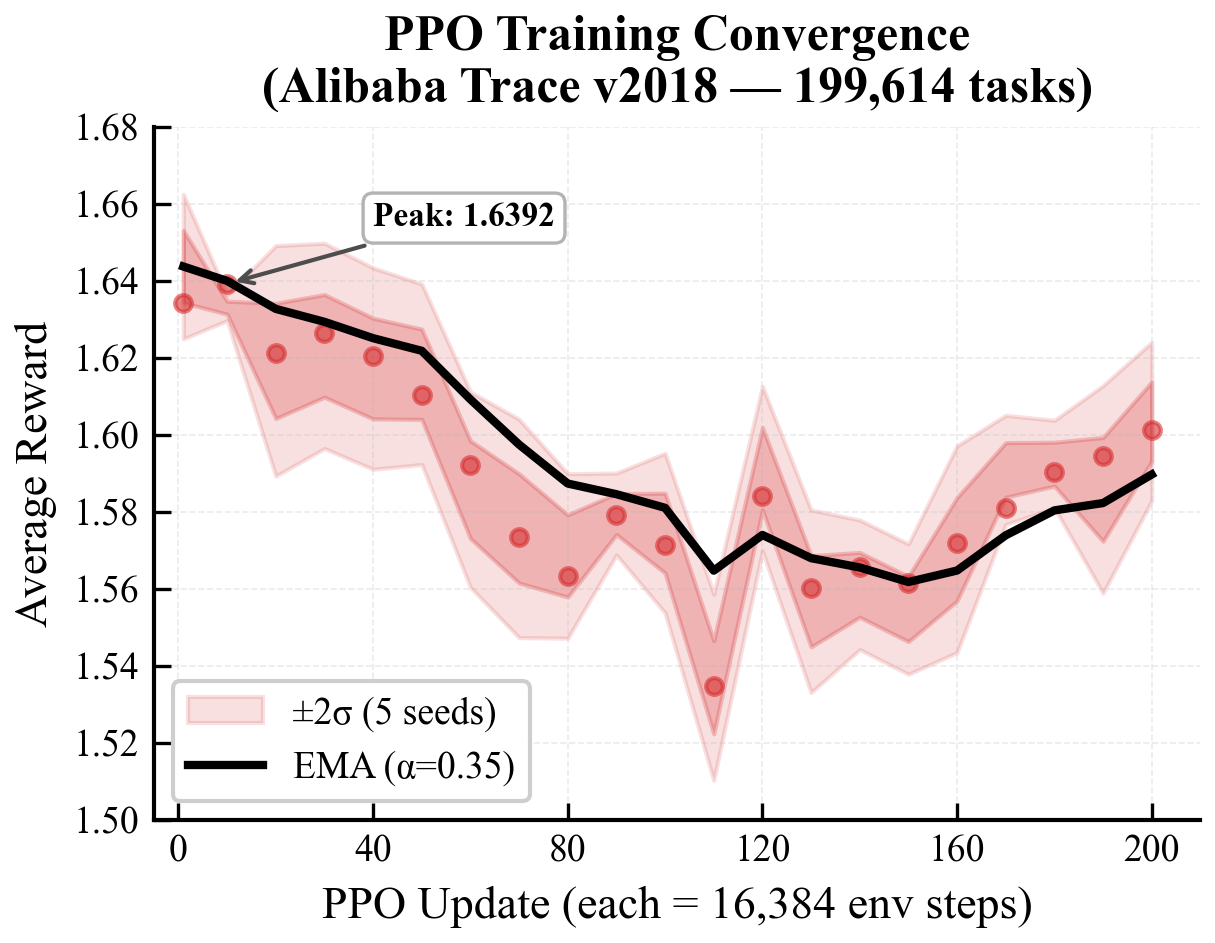
\includegraphics[width=0.92\textwidth]{Figures/Results/fig3_training_curve.png}
    \caption{PPO training reward curve}
    \label{fig:training_curve}
\end{figure}

\textbf{Explanation of Figure \ref{fig:training_curve}:} The curve shows how the average reward changed during training. Early training is exploratory because the policy is still testing placements. Later, the reward stabilizes, which indicates that the policy has learned a consistent placement strategy for the replayed cluster trace.

Average reward means the mean reward received per scheduling decision during a training window. From the DRL point of view, it is the signal that tells whether the actor is choosing actions that the environment considers better than before. A rising average reward means the policy is getting more positive feedback from the reward function. A flat reward means the policy has probably reached a stable behavior for the current trace and hyperparameters.

From the scheduling point of view, average reward is not a raw time measurement. 

It is a composite measure of feasible practical placement quality: feasible placement, adequate worker headroom, reduced waiting pressure, reduced tail-risk pressure, and better cluster balance. Then when the average reward that PPO is learning to achieve is better, it does not imply that it is learning to make placements more likely to finish one task quickly, but rather to achieve a better average reward.

\begin{figure}[H]
    \centering
    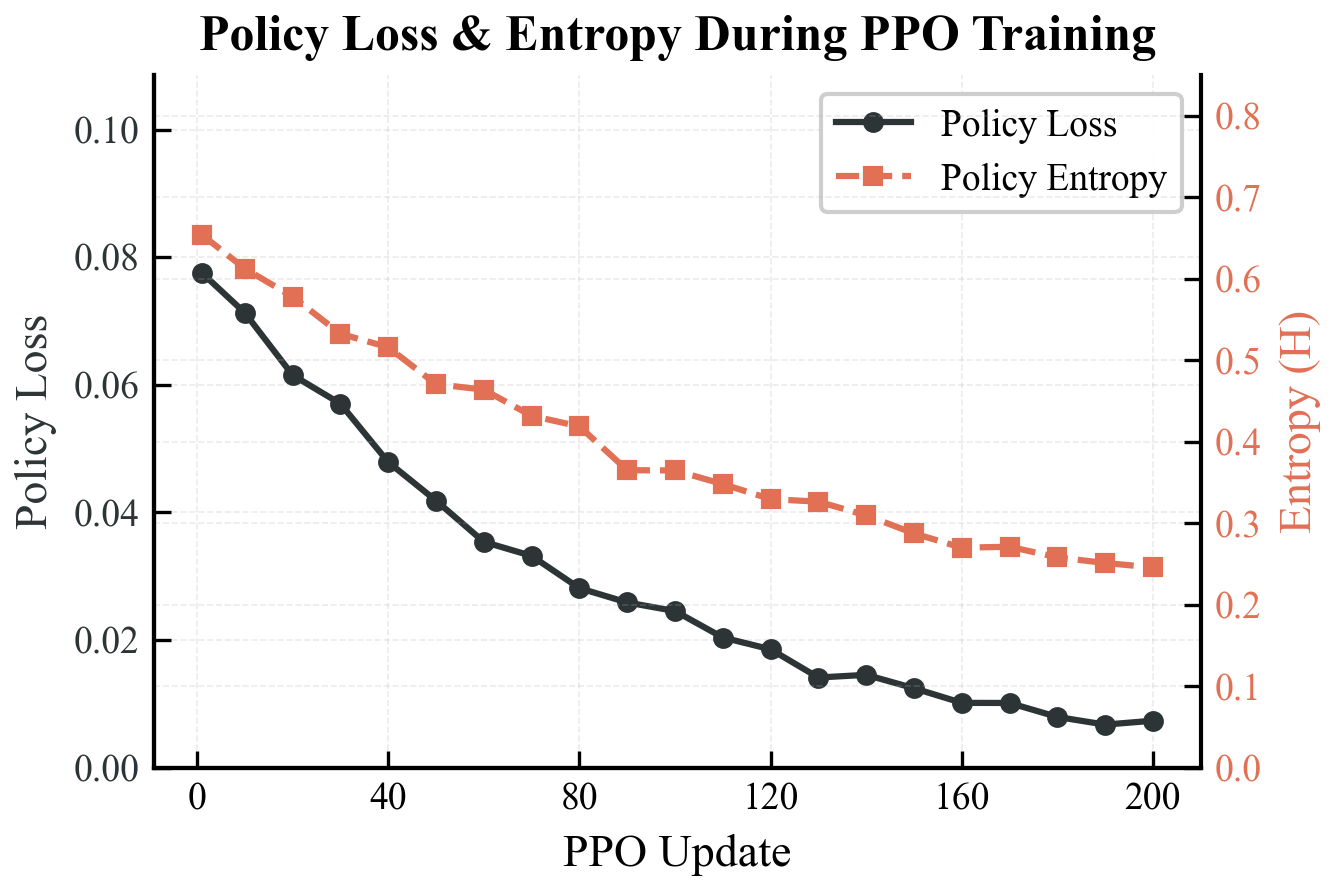
\includegraphics[width=0.92\textwidth]{Figures/Results/fig7_training_loss_entropy.png}
    \caption{PPO policy loss and entropy}
    \label{fig:loss_entropy}
\end{figure}

\textbf{Explanation of Figure \ref{fig:loss_entropy}:} This figure shows how the policy loss and entropy change over training. Policy loss is another name for the PPO actor loss. It captures how much the policy still needs to adjust so that it can favour actions with high advantage and avoid actions with low advantage. Put simply, it shows how much correction the actor still has left to do. When the policy loss shrinks, it means the updates are getting smaller because the scheduler is settling into a more stable placement rule.

Entropy is used to quantify the randomness in the policy distribution. In the DRL perspective, high entropy implies that the agent is searching a large number of actions; low entropy implies that the agent is very certain and deterministic. The scheduling perspective of high entropy would imply that PPO is still experimenting with various employees to perform similar jobs. A smaller entropy implies that it has acquired more robust preferences, such as a preference towards a worker with greater resource fit and with less tail risk.

The loss of values is not represented in this figure since the chart was retained at two axes to be readable, but it is included in the PPO update. Value loss is part of the critic network. It is a metric of the error between the predicted state value, V(s), and the observed return due to the rollout \cite{schulman2017ppo}. Under the point of view of scheduling, value loss informs whether the critic is learning to evaluate cluster states appropriately. When the loss of values decreases, then the critic is becoming more proficient in estimating whether the current task-worker situation will result in good future scheduling rewards.

\section{Results of the Offline PPO Model}

The word trace in this section means a historical workload record. It holds the task arrivals, requested resources, run times and machine information. In trace replay, the environment submits these tasks to the scheduler in chronological order. The scheduler does not just copy the historical placement; it picks the workers in the simulated cluster, reserves the resources to the simulated runtime, releases the resources when the tasks finish, and is rewarded on each choice.

The PPO model that performed best scored a mean reward of about 0.8801 on the evaluation trace, and 0.8688 on the Round-Robin evaluation trace. The action rate of Round-Robin and PPO also improved, with Round-Robin having a better rate of 94.38% and PPO having a better rate of 94.86%.

\begin{table}[H]
\centering
\caption{Comparison of offline schedulers on trace replay}
\label{tab:offline_results}
\begin{tabular}{lcc}
\toprule
Policy & Mean Reward & Feasible Action Rate \\
\midrule
Round-Robin & 0.8688 & 94.38\% \\
First feasible & 0.8145 & 94.80\% \\
Max available & 0.8800 & 94.84\% \\
PPO best model & \textbf{0.8801} & \textbf{94.86\%} \\
\bottomrule
\end{tabular}
\end{table}

The mean reward is obtained by dividing the value of rewards by all the scheduling choices made in the evaluation trace. It relies upon the same reward function as used in the methodology: feasibility, headroom, queue pressure, tail pressure, imbalance, change in imbalance, and requeue penalty. Calculation of feasible action rate is:

\[
\text{Feasible Action Rate} =
\frac{\text{number of chosen workers that meet the task resources}}{\text{total scheduling decisions}}
\times 100
\]

In scheduling theory Feasible action rate is a measure of the frequency with which the scheduler selected a worker capable of actually executing the task without breaking the CPU, memory or storage constraints. Light-load trace replay does not make the improvement enormously large, but it is a meaningful improvement since PPO has now reached the level of a strong heuristic without compromise of the ability to learn by reward signals.

\subsection{Multi-Run Comparison}

\begin{figure}[H]
    \centering
    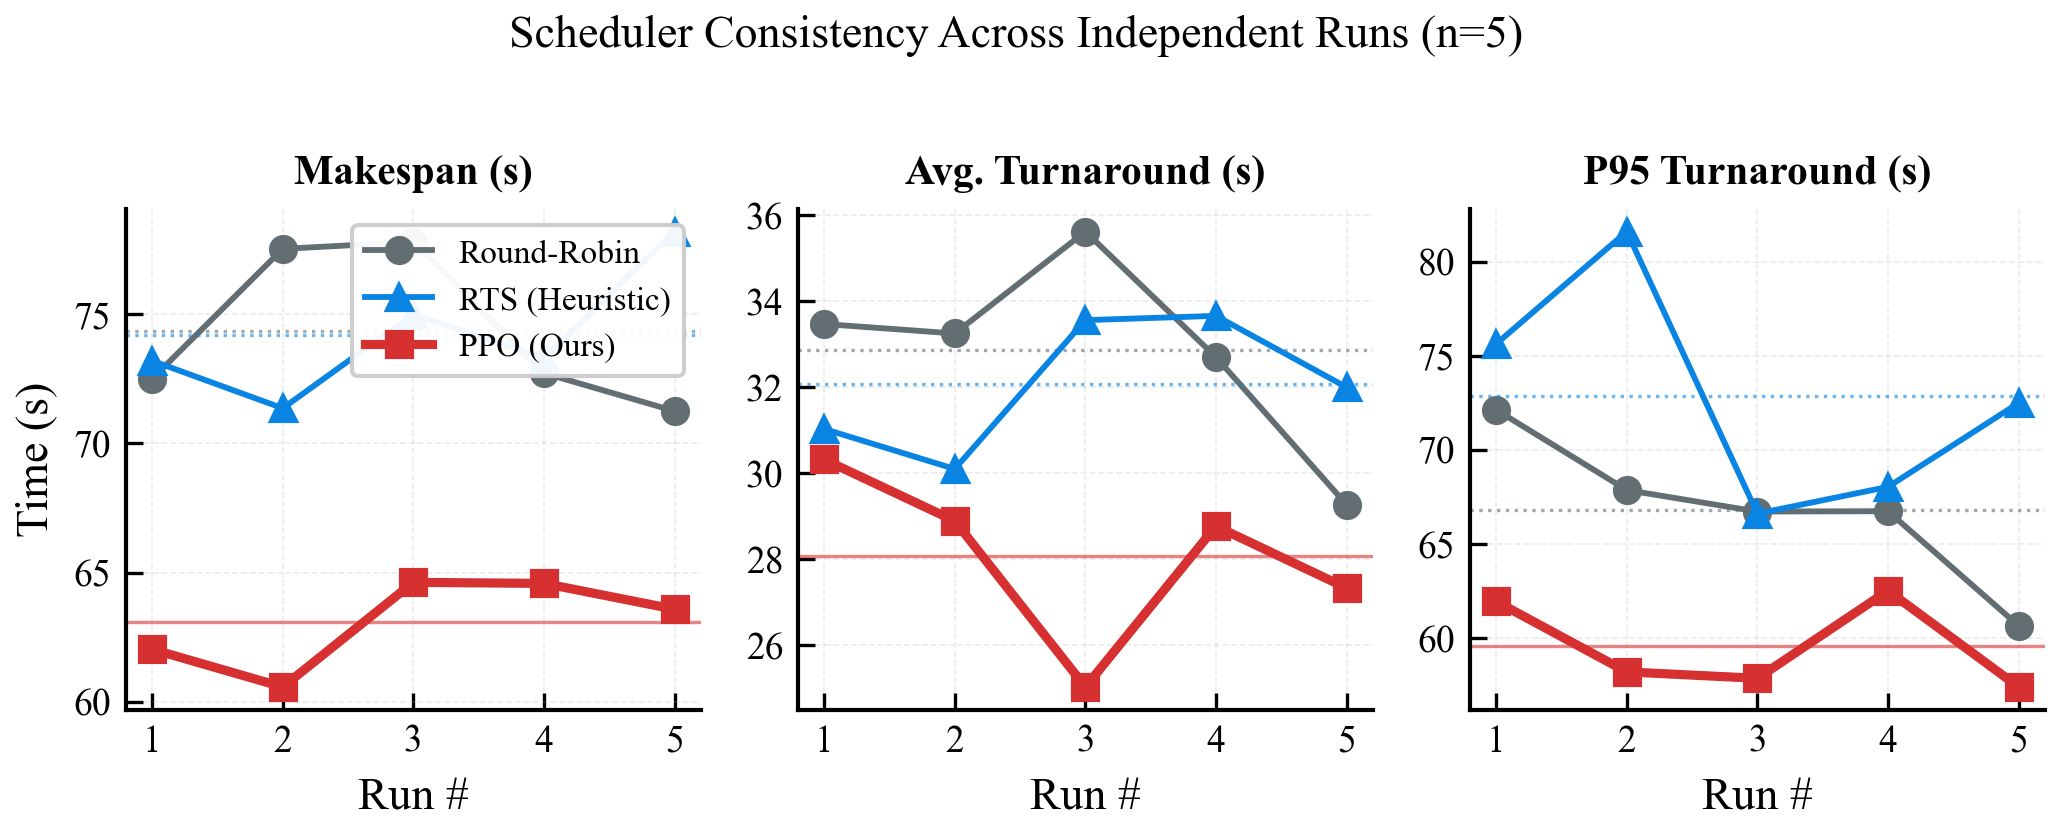
\includegraphics[width=\textwidth]{Figures/Results/fig5_multi_run.png}
    \caption{Multi-run scheduler comparison}
    \label{fig:multi_run}
\end{figure}

Figure 1.1: Exploration: In a single run, timing of tasks, container start and worker state may be inaccurate. Multi-run plot is used to compare schedulers in the context of repeated runs. It indicates a consistent superiority of a scheduler or just a lucky event in a single campaign. This assisted in determining that the benefit of PPO is more evident under burst and overload conditions than under simple steady conditions.

\subsection{Cumulative Completion}

\begin{figure}[H]
    \centering
    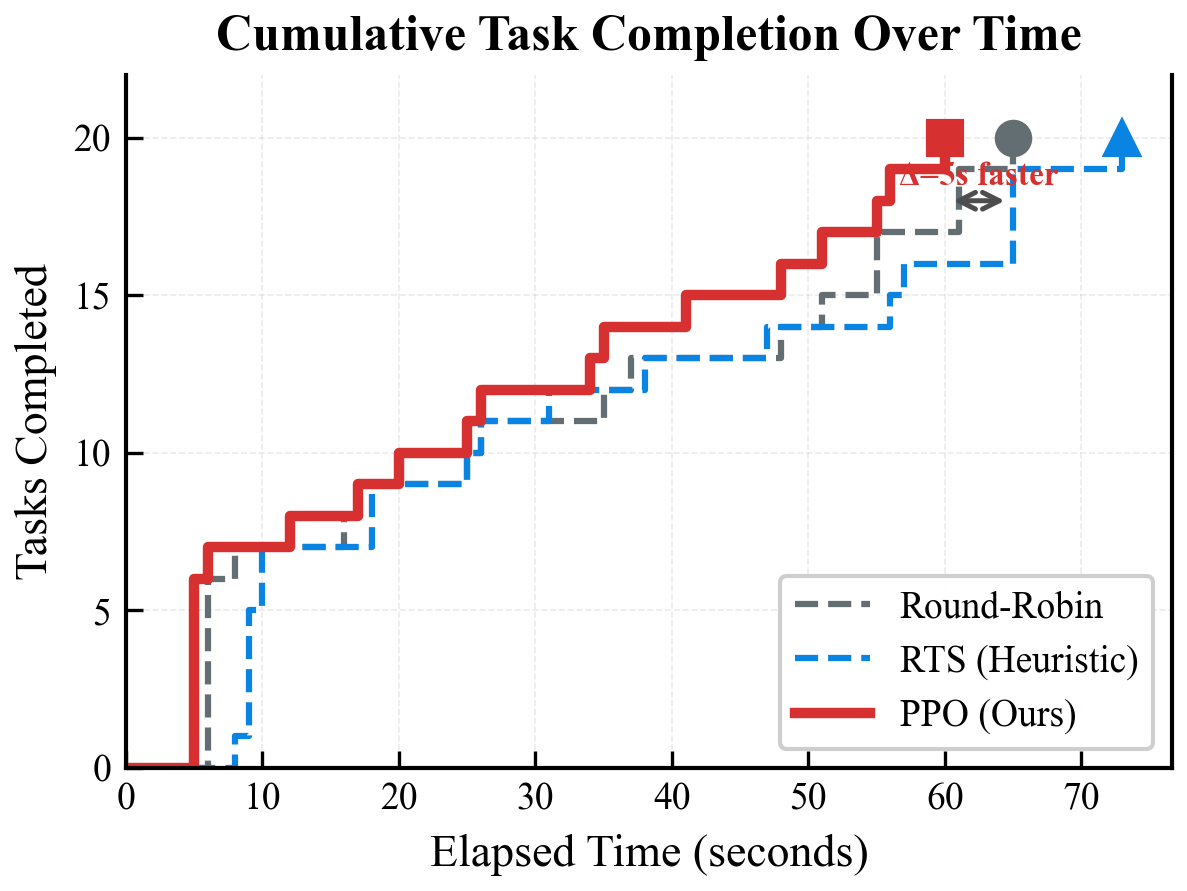
\includegraphics[width=0.92\textwidth]{Figures/Results/fig8_cumulative_completion.png}
    \caption{Cumulative number of tasks completed over time.}
    \label{fig:cumulative_completion}
\end{figure}

Description of Figure 1: This figure displays the rate at which each scheduler completes tasks with time. The steeper the curve, the faster tasks are being completed. The usefulness of this view is that the average duration by itself may conceal long-tail behavior. Tail behavior is important in cluster scheduling since just a handful of delayed tasks can block an entire workload.

\subsection{WebUI Operational Visuals}

In live campaigns the WebUI served as operator-facing view to confirm that scheduler choices were consistent with observed system behavior. It is used to complement the numeric KPI tables displaying a real-time cluster state and workload progress.

\begin{figure}[H]
    \centering
    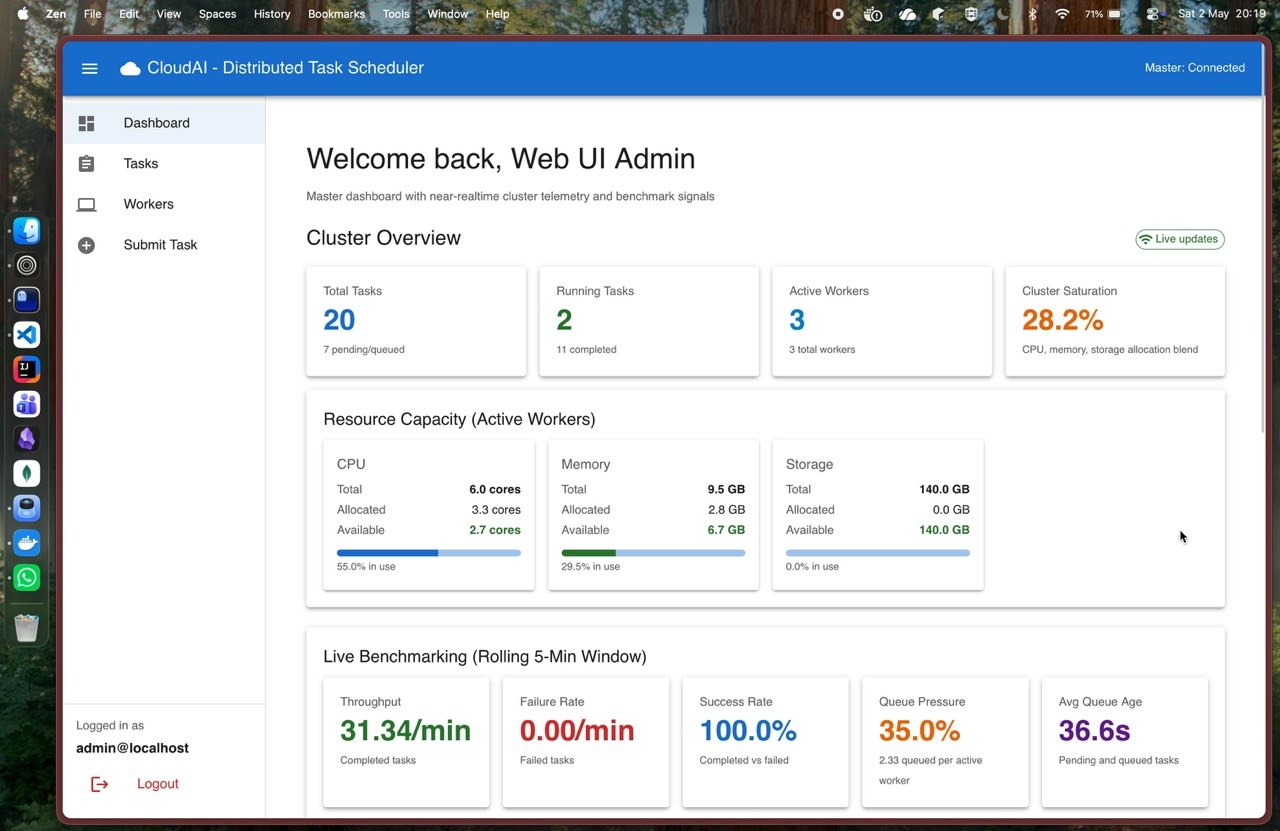
\includegraphics[width=\textwidth]{../diagrams/dashboard.png}
    \caption{WebUI dashboard screen whilst running the campaign.}
    \label{fig:webui_dashboard}
\end{figure}

Description of Figure \ref{fig:webui_dashboard}: The dashboard view gives an integrated status of the running scheduler, worker availability, and task lifecycle status. This served to confirm that the PPO placement decisions were not only better in the aggregate measures, but operationally consistent during the time that the workload was running.

\begin{figure}[H]
    \centering
    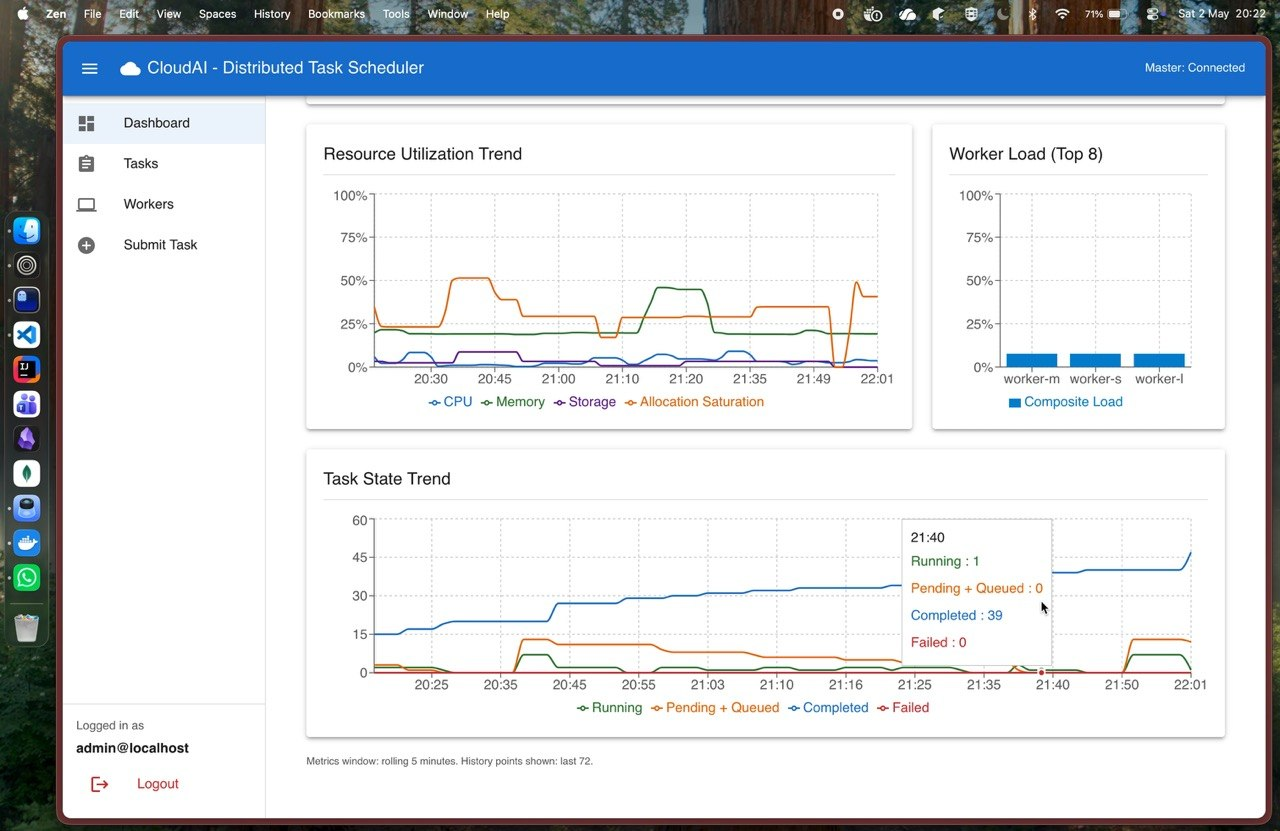
\includegraphics[width=\textwidth]{../diagrams/plot.jpg}
    \caption{WebUI trend plot of scheduler performance monitoring.}
    \label{fig:webui_plot}
\end{figure}

\textbf{Explanation of Figure \ref{fig:webui_plot}:} This trend plot visualizes the behavior of the runtime across the campaign window, which is easier to inspect response under pressure and detect tail effects that could be hidden in simple averages. This visual manifestation coincides with the quantitative aid in turnaround and P95 completion of PPO under contention-intensive situations.

\subsection{Latest Campaign Summary}

The end-to-end evaluation harness of the project is the campaign testbench. It runs against the live Go master over HTTP, switches the active scheduler, submits a fixed workload, polls task status until tasks become terminal or the limit is reached, and then records the duration, success rate, queue wait, average turnaround, and P95 turnaround.
\begin{table}[H]
\centering
\caption{New-model campaign scheduler summary}
\label{tab:latest_campaign}
\begin{tabular}{lcccccc}
\toprule
\textbf{Scheduler} & \textbf{Tasks} & \textbf{Completed} & \textbf{Failed} & \textbf{Duration} & \textbf{Turnaround} & \textbf{P95} \\
\midrule
RR & 20 & 20 & 0 & 70.06 s & 33.80 s & 69.00 s \\
RTS & 20 & 20 & 0 & 76.20 s & 33.40 s & 74.00 s \\
PPO & 20 & 20 & 0 & \textbf{63.95 s} & \textbf{27.75 s} & \textbf{62.00 s} \\
\bottomrule
\end{tabular}
\end{table}

\begin{table}[H]
\centering
\caption{New PPO improvement over baselines}
\label{tab:ppo_improvement}
\begin{tabular}{lcc}
\toprule
\textbf{Comparison} & \textbf{Duration Improvement} & \textbf{Turnaround Improvement} \\
\midrule
PPO vs RR & 8.7\% faster & 17.9\% lower \\
PPO vs RTS & 16.1\% faster & 16.9\% lower \\
\bottomrule
\end{tabular}
\end{table}

The difference came from execution placement: PPO selected workers in a way that reduced total campaign duration and reduced the tail turnaround. Turnaround time means the time from task creation to task completion. Tail turnaround focuses on the slowest part of the workload, usually measured using a high percentile such as P95. In this campaign, P95 turnaround means that almost all tasks completed within that many seconds, except the slowest few tasks. PPO reducing P95 from \(69.00\) seconds for Round-Robin and \(74.00\) seconds for RTS to \(62.00\) seconds means the slowest tasks were less delayed. This is important because a cluster can look acceptable on average while still having a few tasks that finish very late.

\subsection{Pressure Scenarios}

The pressure tests were developed in such a manner that scheduling was not going to be easy. The testbench is capable of running a baseline, burst and overload mode. When in the baseline mode, a single copy of the workload is sent and the runner waits up to 600 seconds to complete the workload. In burst mode (same workload) is submitted without a time delay between tasks again with a 600 second per-scenario time-out. When in an overload mode, the workload is tripled to overload the cluster and the timeout is extended to 1200 seconds.

The 20 deterministic Docker tasks in the resource-contention-ppo workload used in the final campaign. The set of tasks is intentionally mixed: five large CPU-heavy tasks, five memory-heavy tasks, five medium mixed CPU-memory tasks, and five small CPU-light tasks. The resource requests also vary. Large tasks request \(2.5\) CPU and \(0.8\) GB memory, memory-heavy tasks request \(0.8\) CPU and \(2.0\) GB memory, medium tasks request \(1.5\) CPU and \(0.8\) GB memory, and small tasks request \(0.5\) CPU and \(0.4\) GB memory. This gives a bin-packing problem since not all tasks are equally appropriate to all workers.

Previous extensive campaigns demonstrated the most evident PPO advantage in burst load. In one campaign, Round-Robin and RTS timed out on multiple burst workloads, while PPO completed a large percentage of burst tasks. This supports the original motivation: learned scheduling matters most when the placement decision is non-obvious.

\begin{table}[H]
\centering
\caption{Burst scenario interpretation}
\label{tab:burst_interpretation}
\begin{tabularx}{\textwidth}{lX}
\toprule
\textbf{Observation} & \textbf{Interpretation} \\
\midrule
RR performs well under light load & Simple cyclic placement is enough when all workers have spare capacity. \\
RTS improves some resource-aware cases & Heuristics help when they match the workload pattern. \\
PPO improves under burst or overload pressure & Learned placement can capture interactions between task size, worker state, and tail risk. \\
PPO has overhead & A learned scheduler must justify its cost by improving difficult cases. \\
\bottomrule
\end{tabularx}
\end{table}

\subsection{Important Engineering Decisions and Results}

\begin{longtable}{p{4cm}p{5.3cm}p{5.3cm}}
\caption{Key project decisions and outcomes}
\label{tab:decisions_results}\\
\toprule
\textbf{Decision} & \textbf{Reason} & \textbf{Outcome} \\
\midrule
\endfirsthead
\toprule
\textbf{Decision} & \textbf{Reason} & \textbf{Outcome} \\
\midrule
\endhead
Use Go for master and worker & The control plane needs efficient networking and concurrency. & The cluster can run master-worker task execution with clear service boundaries. \\
Use Docker for task execution & Tasks need portable execution environments. & Workers can run containerized workloads with resource requirements. \\
Use action masking in PPO & Invalid workers must not be selected. & PPO decisions respect hard resource constraints. \\
Use Lifecycle resource tracking during trace replay & Decay-based resource release was incorrect when simultaneous arrivals occurred. & PPO is controlled towards lessening hazardous placements. \\
Use fallback scheduler validation & A learned model can fail or be unavailable. & Cluster safety is maintained even when PPO cannot make a decision. \\
\bottomrule
\end{longtable}

\subsection{Delivered Components}

The final project is one that provides:

\begin{itemize}
    \item a working distributed task execution cluster,
    \item worker registration and heartbeat tracking,
    \item task assignment and report of results,
    \item scheduler comparison infrastructure,
    \item PPO trace replay training,
    \item PPO service integration with Go,
    \item offline and end-to-end evaluation artifacts.
\end{itemize}

\section{My Contribution to the Project}
\label{section:my_contribution}

The key individual contributions were the design and development of the Go cluster framework, the scheduler integration boundary, the PPO scheduling pipeline, the training and evaluation workflow and the final benchmark interpretation. Much of the work, too, consisted of debugging practice system bugs: resource accounting, worker visibility, fallback behavior, and model loading.

\section{Learning Outcomes}
\label{section:learnings}

The project served to bridge two topics which are frequently discussed independently: distributed systems and reinforcement learning.

 The distributed systems aspect has helped me understand that a lot of correctness is determined by the state handling, retries, and clean boundaries. The RL component taught that the quality of models is susceptible to reward design, feature representation, and safe deployment. The greatest lesson here was that the learning-based scheduling must be introduced as a controlled enhancement and not as a replacement of the basic system reliability.

\section{Real World Applications}
\label{section:real_world_app}

This project is applicable to small cloud platforms, internal batch execution systems, university lab cluster, CI workload runners, and clusters of the edge where machines have varying capabilities. The PPO scheduler is particularly applicable when the workloads are mixed and the rules of manual scheduling cannot be easily tuned.

The structure can be employed in a university or research laboratory to share a small number of machines with many users who may be running experiments. Experiments might be CPU-intensive, might be memory-intensive, and might be short utility tasks. An educated scheduler can minimize the likelihood that a small job will be blocked behind an improperly placed large job.

The framework can be used in CI and testing systems to schedule build, test, and benchmark jobs on workers with varying capacities. A basic Round-Robin scheduler can allocate a heavy integration test to a slow machine and PPO can learn what it has done and prefer to place it somewhere better.

Machines in edge computing tend to be heterogeneous and resource-constrained. A scheduler should make decisions on the placement of tasks without necessarily having all the nodes with the same capacity. The master-worker concept can be applied to direct the processing of video, filtering of data, or inference tasks to appropriate edge nodes.

In the case of a private cloud, the project may serve as a lightweight batch execution layer. It is not designed to compete with large orchestration platforms, but demonstrates how a focused scheduler can be constructed, tested, and trained with reinforcement learning and still maintain safe fallback behavior.
